\documentclass[tikz,border=5pt]{standalone}

\usepackage{tikz}
\usetikzlibrary{arrows.meta,positioning,calc}

\begin{document}


% Levenshtein DP table for x="kitten" vs y="sitting"
% (rows = prefixes of x, columns = prefixes of y)
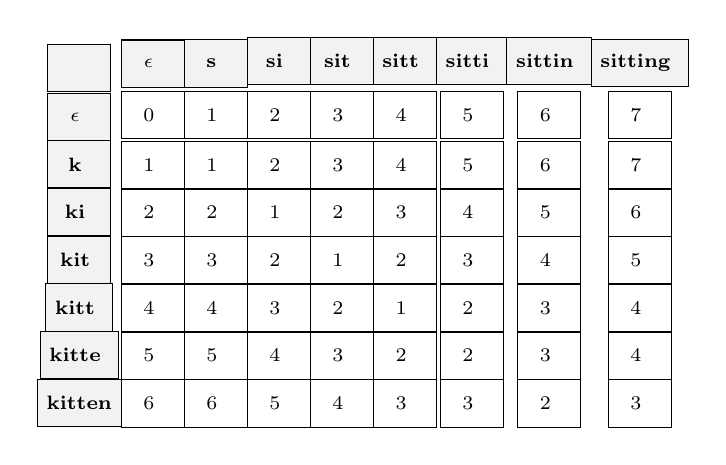
\begin{tikzpicture}[
  font=\scriptsize,
  >=Latex,
  cell/.style={draw, minimum width=8mm, minimum height=6mm, align=center},
  hdr/.style={cell, fill=gray!10, font=\scriptsize\bfseries},
  hi/.style={cell, fill=yellow!25, very thick},
  arrow/.style={->, thick}
]
\usetikzlibrary{matrix,positioning,fit}

% Prefix labels
% x: ε, k, ki, kit, kitt, kitte, kitten
% y: ε, s, si, sit, sitt, sitti, sittin, sitting

\matrix (m) [matrix of nodes,
  nodes in empty cells,
  row sep=-\pgflinewidth,
  column sep=-\pgflinewidth,
  nodes={cell},
  outer sep=0pt
]{
  |[hdr]|      & |[hdr]|$\epsilon$ & |[hdr]|s & |[hdr]|si & |[hdr]|sit & |[hdr]|sitt & |[hdr]|sitti & |[hdr]|sittin & |[hdr]|sitting \\
  |[hdr]|$\epsilon$ & 0 & 1 & 2 & 3 & 4 & 5 & 6 & 7 \\
  |[hdr]|k     & 1 & 1 & 2 & 3 & 4 & 5 & 6 & 7 \\
  |[hdr]|ki    & 2 & 2 & 1 & 2 & 3 & 4 & 5 & 6 \\
  |[hdr]|kit   & 3 & 3 & 2 & 1 & 2 & 3 & 4 & 5 \\
  |[hdr]|kitt  & 4 & 4 & 3 & 2 & 1 & 2 & 3 & 4 \\
  |[hdr]|kitte & 5 & 5 & 4 & 3 & 2 & 2 & 3 & 4 \\
  |[hdr]|kitten& 6 & 6 & 5 & 4 & 3 & 3 & 2 & 3 \\
};

% Highlight one worked cell: D(kit, sit) = 1 computed from neighbours
%% \draw[arrow] (m-4-4.north) -- (m-5-5.south); % diag -> highlighted (kit vs sit)
%% \draw[arrow] (m-4-5.west)  -- (m-5-5.east);  % left -> highlighted
%% \draw[arrow] (m-5-4.south) -- (m-5-5.north); % up -> highlighted

%%\node[above=6mm of m-5-5, align=center] (note) {\bfseries Example cell\\
%$D(\text{kit},\text{sit})=\min\{D(\text{ki},\text{sit}){+}1,\;D(\text{kit},\text{si}){+}1,\;D(\text{ki},\text{si}){+}[t{=}t]\}=1$};

% Emphasise final answer (bottom-right)
%\node[draw, very thick, rounded corners, fit=(m-8-9), inner sep=1pt] {};

\end{tikzpicture}
\end{document}
